\documentclass[a4paper,12pt]{article}
\usepackage{german}
\usepackage{times}
\usepackage{amsmath}
\usepackage{amssymb}
\usepackage{amsfonts}
\usepackage{amsthm}
\usepackage{graphicx}
\usepackage{textcomp}
\usepackage{txfonts}
\usepackage{tikz}
\usepackage{pgfplots}
\usepackage{pgfplotstable}
\usetikzlibrary{arrows}
\usepackage[mode=buildnew]{standalone}
\usepackage{geometry}
\input ../skript/linsys.tex
\geometry{papersize={210mm,297mm},total={160mm,240mm},top=31mm,bindingoffset=15mm}
\begin{document}
\title{"Aquivalentwiderstand von Kubooktaeder und Rhombendodekaeder}
\author{Andreas M"uller}
\date{}
\maketitle
\section{Einleitung}
Die Kirchhoffschen Regeln erlauben, die Str"ome zu berechnen,
die in einem beliebige Netzwerk von Widerst"anden und Spannungsquellen fliessen.
Die lineare Algebra stellt eine Reihe von Hilfsmitteln bereit, die
die Berechnung zu vereinfachen helfen.
Damit wird es m"oglich, auch exotische Netzwerke zu berechnen, zum Beispiel
solche, die als Kanten eines Polyeders auftreten.

Besonders interessant sind nat"urlich die platonischen K"orper Tetraeder, W"urfel,
Oktaeder, Dodekaeder und Ikosaeder, zu denen es in der Aufgabensammlung
einige Information gibt.
Insbesondere sind dort die "Aquivalentwiderst"ande eines mit
1k$\Omega$-Widerst"anden realisierten Kantennetzwerkes f"ur jeden 
platonischen K"orper berechnet worden.

Man stellt dabei auch interessante Zusammenh"ange zwischen sogenannt dualen
K"orpern fest.
Zwei K"orper heissen dual, wenn das Netzwerk der Kanten des einen aus dem des anderen
dadurch hervorgeht, dass man f"ur jede Seitenfl"ache einen Knoten bildet
und genau diejenigen Knoten miteinander "uber eine Kante verbindet, die zu
Seitenfl"achen geh"oren, die an einer Kante zusammenstossen.
Die Dualit"atsbeziehungen f"ur die platonischen K"orper sind:
\begin{center}
\begin{tabular}{ll}
\hline
K"orper&dazu dual\\
\hline
Tetraeder&Tetraeder\\
Hexaeder (W"urfel)&Oktaeder\\
Dodekaeder&Ikosaeder\\
\hline
\end{tabular}
\end{center}

\begin{figure}
\centering
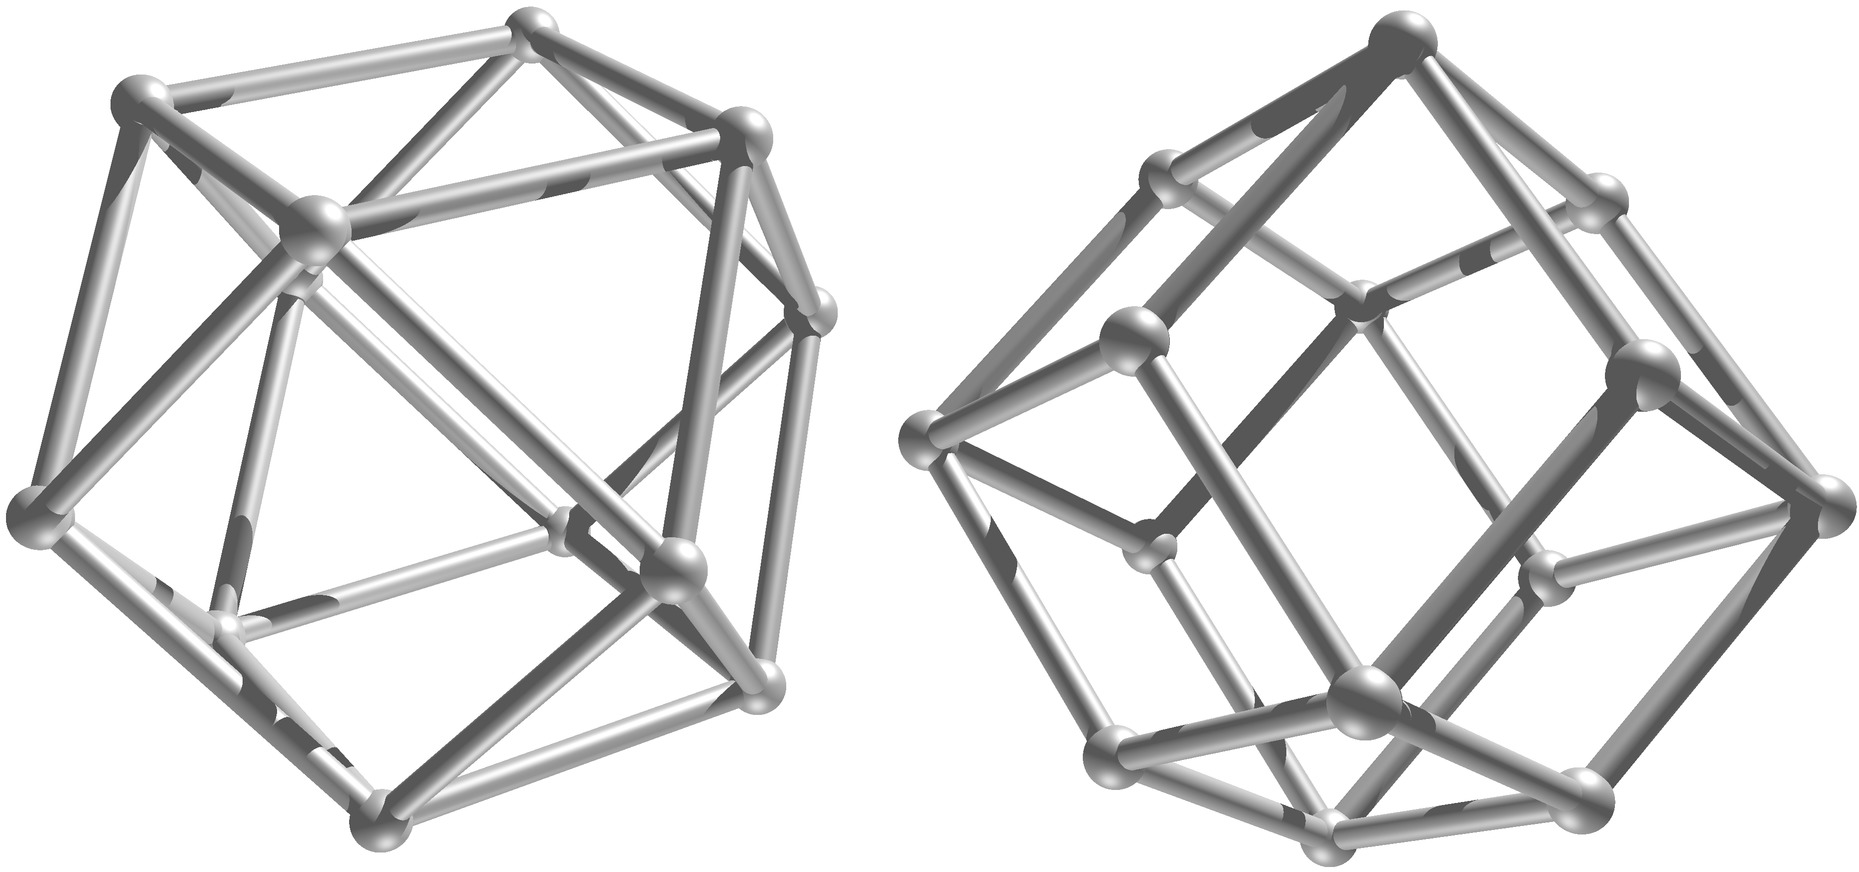
\includegraphics[width=\hsize]{kubooktaeder.jpg}
\caption{Kantennetzwerk von Kubooktaeder (links) und Rhombendodekaeder (rechts)
\label{kantennetzwerke}}
\end{figure}
\begin{figure}
\centering
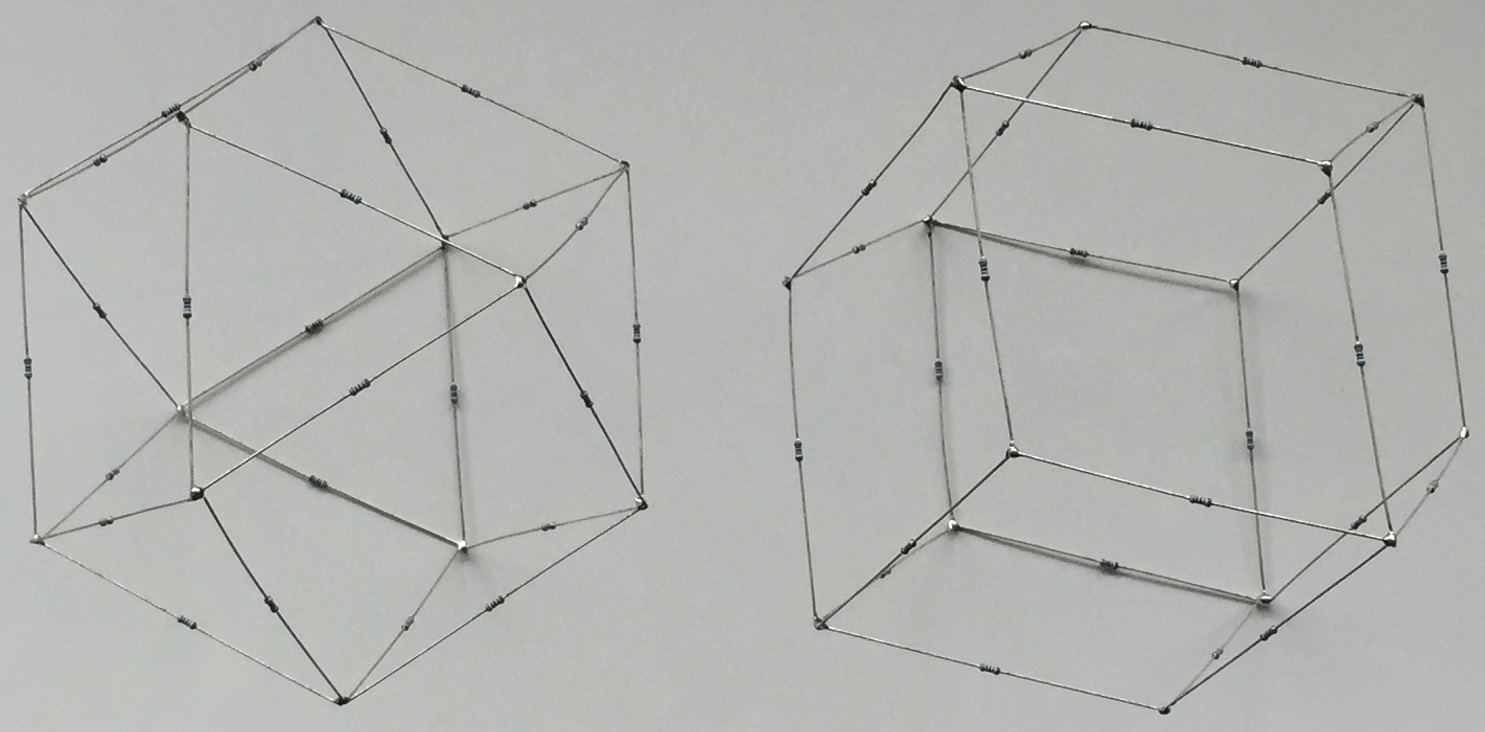
\includegraphics[width=\hsize]{realization.jpg}
\caption{Realisierung des Kantennetzwerks von Kuboktaeder (links)
und Rhombendodekaeder (rechts) mit 1k$\Omega$-Widerst"anden.
\label{realization}}
\end{figure}
Schneidet man einem W"urfel die Ecken durch Ebenen ab, die durch die
Kantenmitten gehen, erh"alt man ein neues Polyeder aus sechs Quadraten
und acht gleichseitigen Dreiecken, ein sogenanntes Kubooktaeder
(Abbildung~\ref{kantennetzwerke}, links).
Es besteht aus acht gleichseitigen Dreiecken und sechs Quadraten.
Den gleichen K"orper k"onnte man auch erhalten, indem man einem Oktaeder
die Ecken durch Ebenen durch die Kantenmitten abschneidet,
was den Namen plausibel macht.
Der dazu duale K"orper ist das Rhombendodekaeder, es besteht aus zw"olf Rhomben.

Die Dualit"at von Kubooktaeder und Rhombendodekaeder spiegelt sich auch in
den Symmetrieeigenschaften der Ecken und Seitenfl"achen.
Beim Kubooktader treffen in allen Ecken vier Kanten zusammen, aber in
verschiedenen Winkeln ($60^\circ$ und $90^\circ$).
Beim Kubooktaeder gibt es also nur eine Art von Ecken, aber zwei Arten von
Seitenfl"achen.
Beim Rhombendodekaeder dagegen gibt es nur eine Art von Seitenfl"achen,
aber zwei verschiedene Arten von Ecken, in denen drei oder vier
Kanten zusammentreffen.
Sie entsprechen nat"urlich den zwei verschiedenen Seitenfl"achen des 
Kubooktaeders.

Man kann das Rhombendodekaeder "ubrigens nicht dadurch erhalten, dass man
einfach die Seitenmitten des Kubooktaeders miteeinander verbindet, denn die
Mitten der quadratischen Seitenfl"achen des Kubooktaeders liegen in der
gleichen Ebene wie zwei der Kanten der Dreiecksfl"achen.
Dies kann man auch in Abbildung~\ref{kantennetzwerke} sehr sch"on sehen.

Umgekehrt ist das Kubooktaeder tats"achlich dadurch realisierbar, dass
man die Seitenmitten des Rhombendodekaeders verbindet, was zum Beispiel
daraus folgt, dass man beim Rhombendodekaeder in jeder $n$-z"ahligen
Ecke (Ecke mit $n$ Kanten) auch eine $n$-fache Rotationssymmetrie hat,
w"ahrend beim Kubooktaeder in den 4-z"ahligen Ecken zwei Quadrate
und zwei Dreiecke zusammenkommen, so dass dort nur eine
$180^\circ$-Rotationssymmetrie m"oglich ist.

\section{Aufgabenstellung}

\newtheorem{aufgabe}{Aufgabe}
\begin{aufgabe}
Man berechne die "Aquivalentwiderst"ande "uber eine Kante eines mit
1k$\Omega$-Widerst"anden realisierten Kubookateders und eines Rhombendodekaeders.
\end{aufgabe}

{\parindent0pt \bf Wettbewerbsbedingungen:}
\begin{enumerate}
\item
Die L"osung muss so dokumentiert sein, dass sie ohne weitere Hilfsmittel
nachvollziehbar ist.
\item
Es ist zul"assig, ein Computerprogramm zu verwenden, welches aber ebenfalls
soweit dokumentiert sein muss, dass man es nicht selbst kompilieren oder
ausf"uhren muss um zu verstehen, wie es funktioniert.
\item
Zur Kontrolle der eigenen L"osung stehen die Realisationen der beiden
Netzwerke zum Nachmessen zur Verf"ugung (Abbildung~\ref{realization}).
\item
Eingabefrist: 1.~November 2015, 00:00 Uhr.
\item
"Uber den Wettbewerb wird keine Korrespondenz gef"uhrt.
\end{enumerate}

\section{L"osung}
Die Theorie zur L"osung der vorliegenden Art von Problemen ist
im wesentlichen im Skript erkl"art, in der Vorlesung haben wir
uns vor allem auf das Aufstellen der Kirchhoff-Gleichungen 
konzentriert.
Damit man den Widerstand bestimmen kann, muss man irgendwie eine
Spannungsquelle anschliessen und die entstehende Spannungs- und Stromverteilung
berechnen.
Dies ist auf verschiedene Arten m"oglich, und ist in Abschnitt~\ref{quelle}
diskutiert.

Beide Netzwerke haben 24 Kanten, f"ur die L"osung m"ussen also etwas
unhandliche Gleichungssysteme gel"ost werden.
Abschnitt~\ref{vereinfachung} beschreibt, wie man die Netzwerke und
damit die Gleichungssysteme vereinfachen kann.

Das im Skript beschriebene L"osungsverfahren verlangt zun"achst,
dass die Matrix $\partial$ der Verbindungen im Netzwerk aufgestellt
wird, sie ergibt dann bereits die Knotengleichung $\partial I=0$.
Aus $\partial$ kann eine minimale Menge von Maschen gewonnen werden,
die die Spalten der Matrix $Z$ bilden.
Die Maschengleichungen sind dann
\[
Z^tRI=Z^te,
\]
wobei $e$ der Vektor der Spannungen in den Kanten ist.
Da die Zeilen von $\partial$ linear abh"angig sind, kann man
einfach die letzte Zeile weglassen, so dass zusammen mit der Matrix $Z^tI$
eine regul"are quadratische $n\times n$-Matrix entsteht.


\subsection{Spannungsquellen\label{quelle}}
Um den "Aquivalentwiderstand "uber eine Kante zu ermitteln, muss
eine Spannungsquelle hinzugef"ugt werden, die im Netzwerk einen
Strom hervorruft.
Wir nehmen im folgenden an, dass der Widerstand zwischen den Knoten
$1$ und $2$ ermittelt werden soll.

Man kann zum Beispiel in den Knotengleichungen $\partial I=0$
die rechte Seite modifizieren.
In der ersten Knotengleichung setzt man die rechte Seite auf $i_0$,
in der zweiten auf $-i_0$.
Die L"osung des Gleichungssystems liefert dann den die Spannung $u_0$ zwischen
den beiden Knoten $1$ und $2$, und damit kann der "Aquivalent-Widerstand
als $u_0/i_0$ berechnet werden.

Die zweite M"oglichkeit ist, dass man dem Netzwerk eine zus"atzliche
Kante hinzuf"ugt, die eine Spannungsquelle enth"alt. 
Das Gleichungssystem wird dadurch etwas gr"osser, man kann zum
Beispiel die Masche bestehend aus der interessierenden Kante und
der Spannungsquelle hinzuf"ugen.
Ist $i_0$ der Strom in dieser Masche und $u_0$ die Spannung der
Spannungsquelle, dann kann man den Widerstand wieder als $u_0/i_0$
finden.

\begin{figure}
\centering
\includestandalone{spannungsquelle}
\caption{Spannungsquelle in der ersten Kante, $R$ ist der Wiederstand
der Kante, $R'$ ist der Widerstand des Netzwerkes ohne die Kante.
\label{spannungsquelle}}
\end{figure}
Die geringsten Modifikationen am Gleichungssystem sind n"otig, wenn
man die Spannungsquelle mit mit Spannung $u_0$ in die interessierende
Kante einbaut.
Die Spannung $u_0$ dieser Spannungsquelle taucht dann in der
der Kante entsprechenden Position in $e$ auf.
Der resultierende Strom $i_0$ liefert den Widerstand $R+R'=u_0/i_0$
oder $R'=u_0/i_0-R$.
Der gesucht Widerstand $r$ ist jedoch die Parallelschaltung von $R$ und $R'$,
also
\[
\frac1r=\frac1{R}+\frac1{u_0/i_0-R}.
\]

\subsection{Vereinfachungen\label{vereinfachung}}
Die Gleichungssystem zur Berechnung des Widerstandes sind ziemlich gross,
immerhin haben beide Netzwerke 24 Kanten und damit mindestens im Prinzip 
24 unbekannte Str"ome oder Spannungen, die zu bestimmen sind.
\begin{figure}
\centering
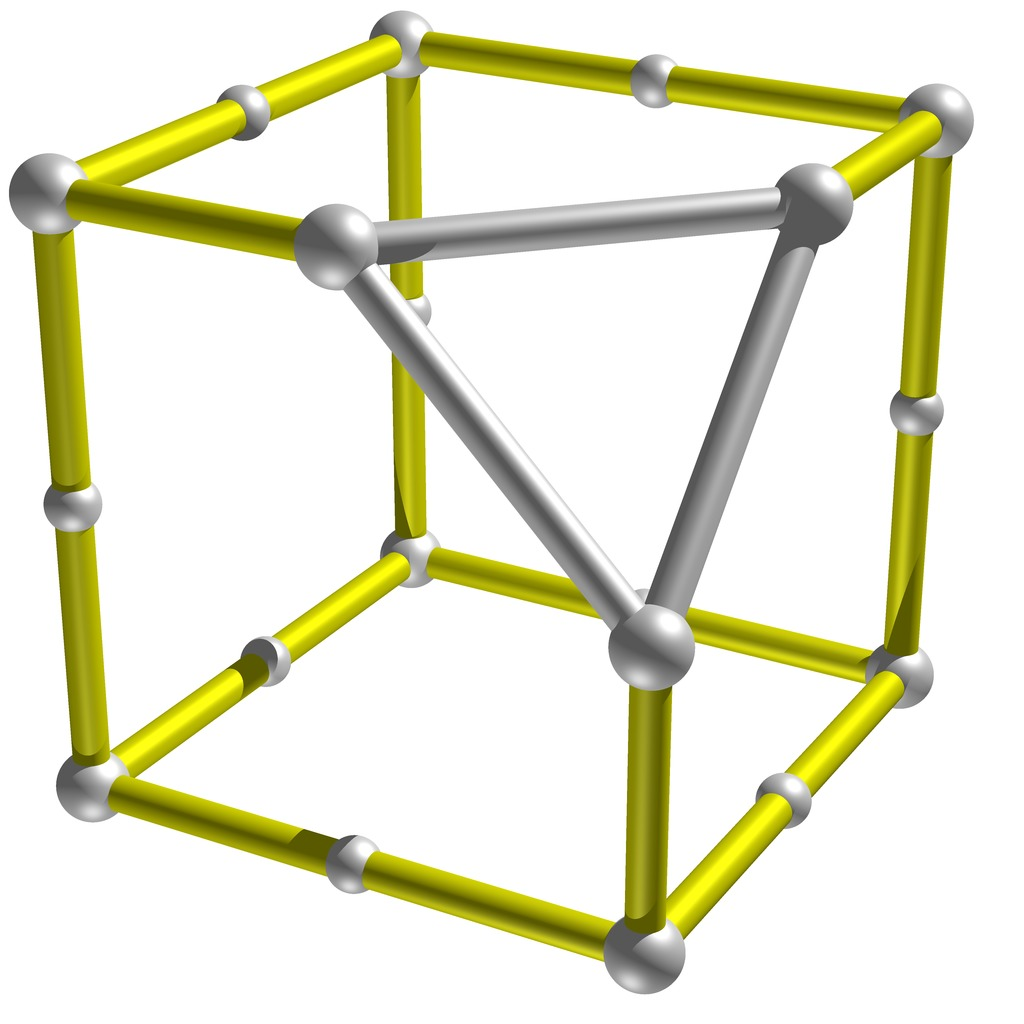
\includegraphics[width=0.45\hsize]{vereinfachung.jpg}
\quad
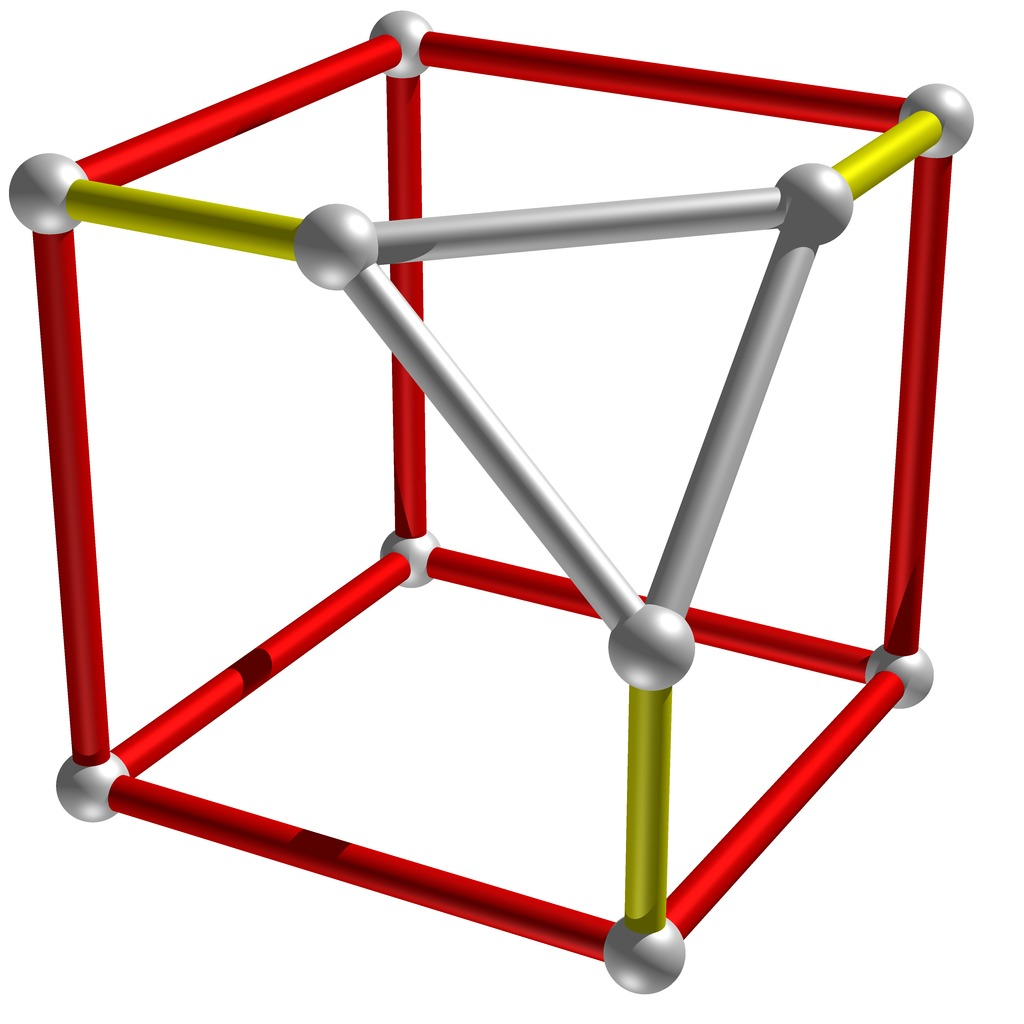
\includegraphics[width=0.45\hsize]{vereinfachung2.jpg}
\caption{Vereinfachung des Kubooktaeders mit Hilfe der Stern-Dreieck-Methode.
F"unf Dreiecke werden durch die gelben Sterne ersetzt (links),
danach k"onnen zwei gelbe Kanten in Serie durch eine rote Kante
ersetzt werden (rechts).
\label{wuerfel}}
\end{figure}
\begin{figure}
\centering
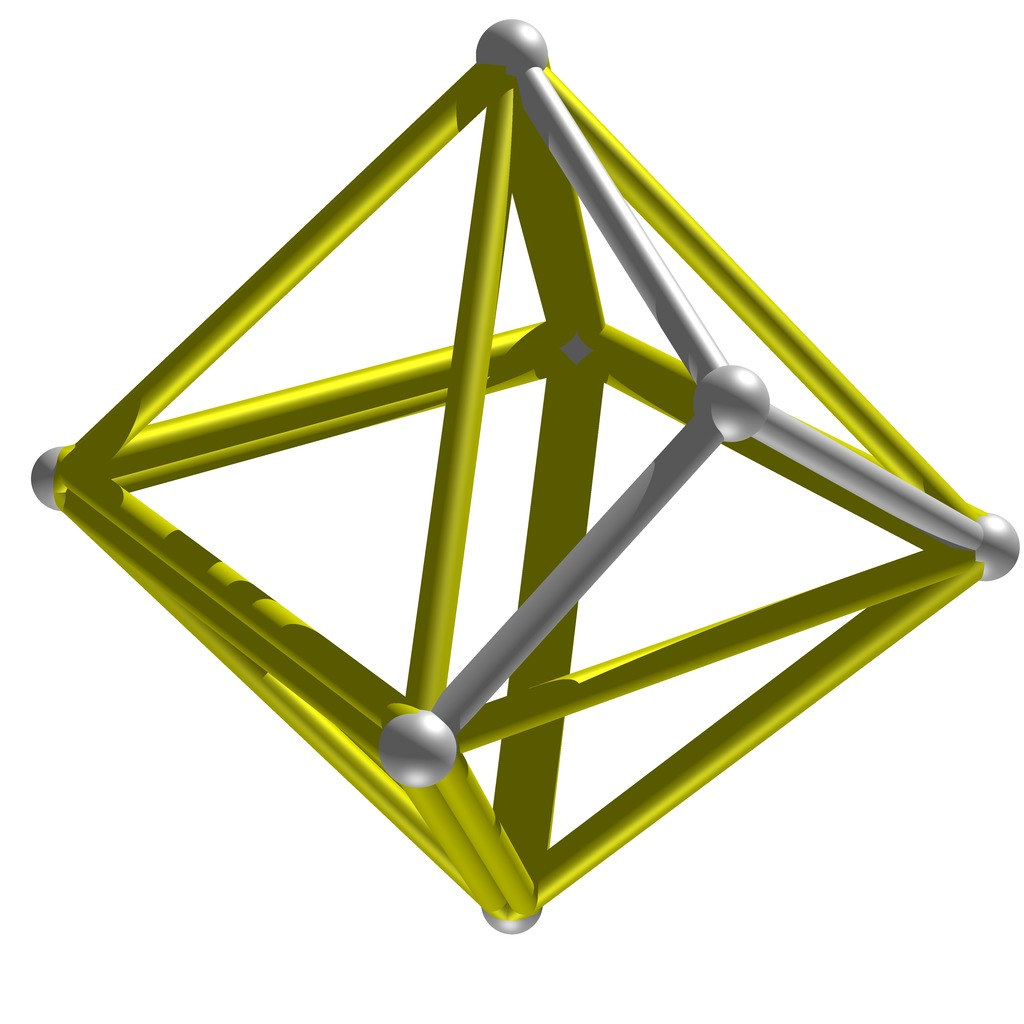
\includegraphics[width=0.45\hsize]{oktaeder.jpg}
\quad
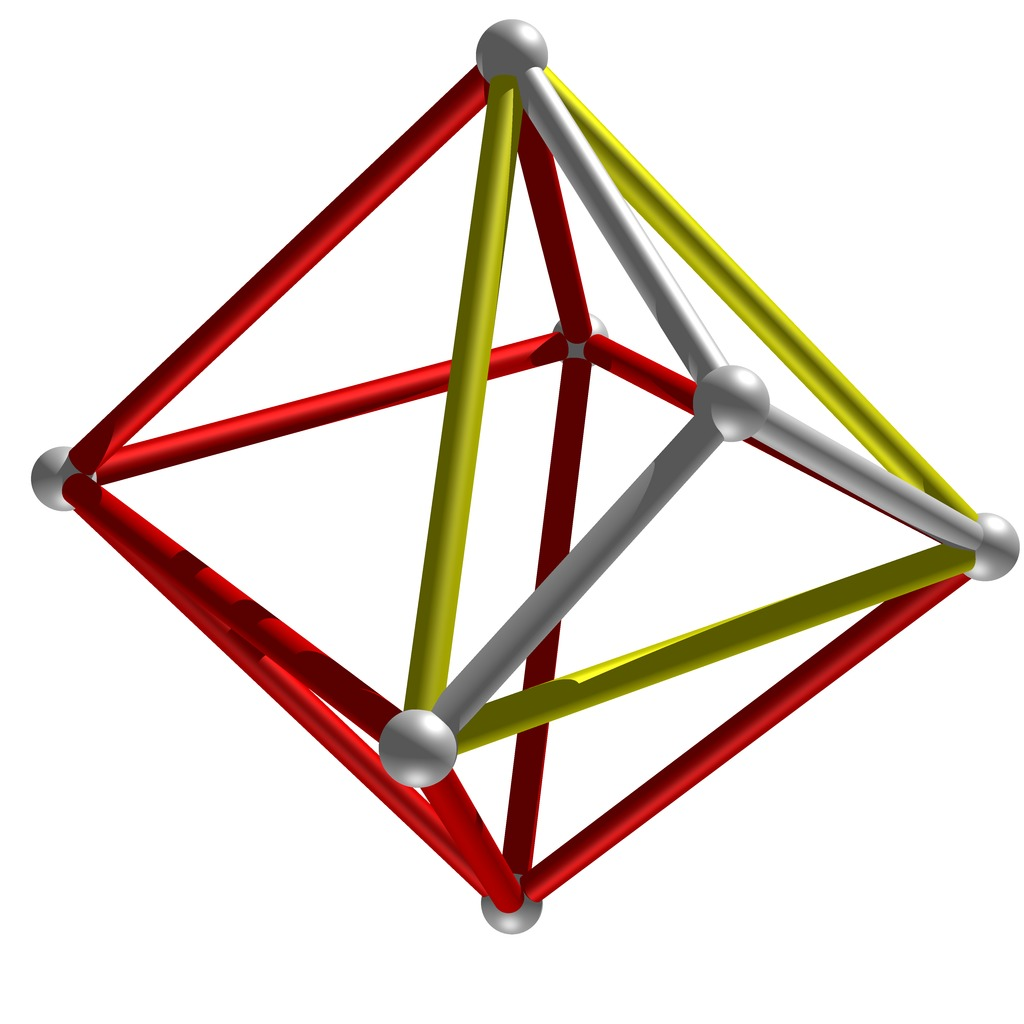
\includegraphics[width=0.45\hsize]{oktaeder2.jpg}
\caption{Vereinfachung des Rhombendodekaeders mit Hilfe der
Stern-Dreieck-Methode.
F"unf Sterne werden ersetzt durch die gelben Dreiecke (links), und
anschliessend die parallelen Kanten zu einer roten Kante zusammengefasst
(rechts).
\label{oktaeder}}
\end{figure}
Ersetzt man im Kubooktaeder jedes Dreieck durch einen Stern
wird daraus ein W"urfel.
Ebenso wird aus dem Rhombendodekaeder ein Oktaeder, wenn man
jeden Stern durch ein Dreieck ersetzt.
W"urfel und Oktaeder sind ebenfalls dual zueinander, haben aber 
nur zw"olf Kanten und acht bzw.~sechs Ecken, die Gleichungen
f"ur diese beiden Netzwerke w"aren also deutlich einfacher.
Ausserdem bleibt die Eigenschaft erhalten, dass alle Widerst"ande
gleich gross sind.

Allerdings bringen diese Transformationen auch die Kante zum
verschwinden, "uber die der "Aquivalent-Widerstand bestimmt werden
soll.
Die Transformation muss daher im Falle des Kubooktaeders ein Dreieck 
und im Falle des Rhombendodekaeders einen Stern unber"uhrt lassen.
Wie die Abbildungen \ref{wuerfel} und \ref{oktaeder}
zeigen, werden im resultierenden Netzwerk drei verschiedene Widerstandswerte
auftreten.

Nadja Rutz hat in Ihrer L"osung beide Netzwerke in der oben genannten
Art verwendet, w"ahrend Matthias Schneider die Transformation nur beim
Kubooktaeder durchf"uhrte.

Die Vereinfachungen k"onnten aber noch weiter getrieben werden.
Die Ersetzung eines Sterns durch ein Dreieck ist in Abbildung~\ref{stern3}
dargestellt.

\begin{figure}
\centering
\includestandalone{stern}
\caption{Stern-Dreieck-Ersetzung
\label{stern3}}
\end{figure}
Die Ersetzung eines Sterns durch ein Dreieck ist auch f"ur $n$-Ecke
m"oglich, mindestens f"ur ungerade $n$.
F"ur gerade $n$ sind zus"atzliche Bedingungen n"otig.
Man die Gleichungen f"ur die Widerst"ande $R_i$ ablesen:
\begin{equation}
\begin{linsys}{3}
R_1&+&R_2& &   &=&\displaystyle\biggl(\frac1{r_1}+\frac1{s-r_1}\biggr)^{-1}\\
   & &R_2&+&R_3&=&\displaystyle\biggl(\frac1{r_2}+\frac1{s-r_2}\biggr)^{-1}\\
R_1& &   &+&R_3&=&\displaystyle\biggl(\frac1{r_3}+\frac1{s-r_3}\biggr)^{-1}
\end{linsys}
\label{dreieck}
\end{equation}
mit $s=r_1+r_2+r_3$.
Es ist wohlbekannt, dass das Gleichungsystem die L"osung
\[
R_i=\frac{r_1r_2r_3}{s}\cdot\frac1{r_i}
\]
hat.

Eine analoge Ersetzung ist auch m"oglich f"ur ein $n$-Eck.
Die Gleichungen, die (\ref{dreieck}) entsprechen, werden dabei zu
\begin{equation}
\begin{linsys}{6}
R_1&+&R_2& &   & &   & &   & &   &=&
	\displaystyle\biggl(\frac1{r_1}+\frac1{s-r_1}\biggr)^{-1}\\
   & &R_2&+&R_3& &   & &   & &   &=&
	\displaystyle\biggl(\frac1{r_2}+\frac1{s-r_2}\biggr)^{-1}\\
   & &   & &R_3&+&R_4& &   & &   &=&
	\displaystyle\biggl(\frac1{r_3}+\frac1{s-r_3}\biggr)^{-1}\\
   & &   & &   & &\ddots& &\ddots& &   & &\\
R_1& &   & &   & &   & &   &+&R_n&=&
	\displaystyle\biggl(\frac1{r_n}+\frac1{s-r_n}\biggr)^{-1}
\end{linsys}
\label{nstern}
\end{equation}
Die linke Seite kann als lineares Gleichungssystem mit der Koeffizientenmatrix
\[
A_n=\begin{pmatrix}
     1&     1&     0& \dots&     0&     0\\
     0&     1&     1& \dots&     0&     0\\
     0&     0&     1& \dots&     0&     0\\
\vdots&\vdots&\vdots&\ddots&\vdots&\vdots\\
     0&     0&     0& \dots&     1&     1\\
     1&     0&     0& \dots&     0&     1
\end{pmatrix}
\]
geschrieben werden.
Die $n\times n$-Matrix $A_n$ ist nur f"ur ungerade $n$ invertierbar.
Man kann n"amlich die Determinante mit Hilfe des Entwicklungssatzes berechnen:
\begin{align*}
\det(A_n)
&=
\left|
\begin{matrix}
     1&     1& \dots&     0&     0\\
     0&     1& \dots&     0&     0\\
\vdots&\vdots&\ddots&\vdots&\vdots\\
     0&     0& \dots&     1&     1\\
     0&     0& \dots&     0&     1
\end{matrix}
\right|
-(-1)^n
\left|
\begin{matrix}
     1&     0& \dots&     0&     0\\
     1&     1& \dots&     0&     0\\
     0&     1& \dots&     0&     0\\
\vdots&\vdots&\ddots&\vdots&\vdots\\
     0&     0& \dots&     1&     1
\end{matrix}
\right|
=1-(-1)^n
=\begin{cases}
2&\quad\text{$n$ ungerade}\\
0&\quad\text{$n$ gerade}
\end{cases}
\end{align*}
F"ur ungerade $n$ ist also die Ersetzung eines $n$-Sterns durch ein $n$-Eck
oder umgekehrt immer auf eindeutige Art m"oglich.

F"ur gerade $n$ ist die Matrix $A_n$ nicht invertierbar, damit die
Gleichungen (\ref{nstern}) l"osbar sind, m"ussen die rechten Seiten eine
zus"atzliche lineare Bedingung erf"ullen.
Nehmen wir an, dass die Bedingung die Form
\[
\sum_{i=1}^nb_i\biggl(\frac1{r_i}+\frac1{s-r_i}\biggr)^{-1}=0
\]
mit Koeffizienten $b_i$ hat.
Da $A_n$ nicht regul"ar ist, m"ussen alle Spalten von $A_n$ die
Bedingung erf"ullen, es muss also gelten
\[
A^tb=0\qquad \text{mit}\;
b=\begin{pmatrix}b_1\\\vdots\\b_n\end{pmatrix}.
\]
Das Gleichungssystem  kann mit dem Gaussalgorithmus gel"ost werden:
\begin{align*}
\begin{tabular}{|
>{$}c<{$}
>{$}c<{$}
>{$}c<{$}
>{$}c<{$}
>{$}c<{$}
>{$}c<{$}
>{$}r<{$}
|}
\hline
     1&     0&     0&     0& \dots&     0&     1\\
     1&     1&     0&     0& \dots&     0&     0\\
     0&     1&     1&     0& \dots&     0&     0\\
     0&     0&     1&     1& \dots&     0&     0\\
\vdots&\vdots&\vdots&\vdots&\ddots& \dots&\vdots\\
     0&     0&     0&     0& \dots&     1&     0\\
     0&     0&     0&     0& \dots&     1&     1\\
\hline
\end{tabular}
&\rightarrow
\dots
\rightarrow
\begin{tabular}{|
>{$}c<{$}
>{$}c<{$}
>{$}c<{$}
>{$}c<{$}
>{$}c<{$}
>{$}c<{$}
>{$}r<{$}
|}
\hline
     1&     0&     0&     0& \dots&     0&     1\\
     0&     1&     0&     0& \dots&     0&    -1\\
     0&     0&     1&     0& \dots&     0&     1\\
     0&     0&     0&     1& \dots&     0&    -1\\
\vdots&\vdots&\vdots&\vdots&\ddots&\ddots&\vdots\\
     0&     0&     0&     0& \dots&     1&     1\\
     0&     0&     0&     0& \dots&     0&     0\\
\hline
\end{tabular}
\end{align*}
Man kann ablesen, dass $\operatorname{Rang}A_n=n-1$ ist, und dass f"ur
die $b_i$ die Zahlen $b_i=(-1)^i$ eine L"osung sind.
Das Gleichungssystem (\ref{nstern})  ist
genau dann l"osbar , wenn die rechten Seiten die Bedinung
\begin{equation}
\sum_{i=1}^n (-1)^i \biggl(\frac1{r_i}+\frac1{s-r_i}\biggr)^{-1}=0
\label{condition}
\end{equation}
erf"ullt ist.
Sie ist insbesondere dann erf"ullt, wenn die Widerst"ande $r_i$
alle gleich sind.
%Durch "Ubergang zu Leitf"ahigkeiten k"onnen analoge Gleichungen f"ur
%die Ersetzung in der umgekehrten Richtung formuliert werden.

Im Falle des Rhombendodekaeders, das zum gr"ossten Teil bereits in
ein Oktaeder umgewandelt wurde wie in Abbildung~\ref{oktaeder},
sind zwei 4-Sterne vorhanden, aus identischen Widerst"anden
vorhanden.
Ein $n$-Stern aus identischen Widerst"anden $R$ kann durch ein $n$-Eck
aus ebenfalls identischen Widerst"anden $r$ ersetzt werden, und es
gilt
\begin{align*}
\frac{1}{2R}
&=
\frac{1}{r}+\frac{1}{(n-1)r}
\\
\frac{1}{2R}
&=
\frac{1}{r}
\biggl(1+\frac1{n-1}\biggr)
=
\frac{1}{r}\frac{n}{n-1}
\\
r&=\frac{2nR}{n-1}.
\end{align*}
Damit l"asst sich der 4-Stern ebenfalls eliminieren.

Durch Anwendung dieser Ersetzungen kann das Netzwerk sukzessive 
vereinfacht werden bis nur noch die Verbindung zwischen den zwei
ausgew"ahlten Ecken "ubrig bleibt.

\subsection{Vermutungen}
Matthias Schneider hat aufgrund der numerischen Resultate vermutet,
dass der Widerstand sich direkt aus der Anzahl $E$ der Ecken und
und der Anzahl $K$ der Kanten ermitteln l"asst:
\[
R=\frac{E-1}{K}.
\]
So eine Formel kann nat"urlich nur zutreffen, wenn alle Kanten
des Netzwerks gleichwertig sind. 
Die vorliegenden Netzwerke erf"ullen diese Bedingung, aber
auch die Kanten der platonischen K"orper (regelm"assigen Polyeder),
und die Vermutung trifft auch dort zu.

Kubooktaeder und Rhombendodekaeder sind zueinander dual.
Bezeichnen wir die die Fl"achen\-, Kanten- und Ecken-Zahl des
Kubooktaeders mit $F_1$, $K_1$ und $E_1$ und die entsprechenden
Zahlen des Rhombendodekaeders mit $F_2$, $K_2$ und $E_2$, dann
bedeutet die Dualit"at, dass gilt
\begin{equation}
\begin{aligned}
F_1&=E_2,&\qquad
K_1&=K_2,&\qquad
E_1&=F_2.
\end{aligned}
\label{dualitaet}
\end{equation}
Der Eulersche Polyeder-Satz besagt, dass f"ur die Zahlen $F$, $K$ und $E$
jedes Polyeders die Beziehung
\begin{equation}
E-K+F=2
\qquad
\Rightarrow
\qquad
E+F-2=K
\label{euler}
\end{equation}
gilt.
Die Widerst"ande sind gem"ass obiger Vermutung $R_i=(E_i-1)/K_i$.
und deren Summe wird unter Verwendung von (\ref{dualitaet}) 
und (\ref{euler})
\begin{align*}
R_1+R_2
&=
\frac{E_1-1}{K_1}
+
\frac{E_2-1}{K_2}
=
\frac{E_1+F_1-2}{K_1}
=
\frac{K_1}{K_1}=1.
\end{align*}
Auch diese Beziehung kann nat"urlich nur gelten, wenn alle Kanten den
gleichen Widerstand haben.

Bei dualen Netzwerk k"onnen wir zu jeder Kante im einen Netzwerk die dazu
geh"orige duale Kante im dualen Netzwerk identifizieren.
Selbst wenn die Widerst"ande der Kanten verschieden sind, kann man
eine einfache Beziehung zwischen den "Aquivalentwiderst"anden zueinander
dualer Kanten beweisen.

\end{document}
